%%%%%%%%%%%%%%%%%%%%%%%%%%%%%%%%%%%%%%%%%
% Short Sectioned Assignment LaTeX Template Version 1.0 (5/5/12)
% This template has been downloaded from: http://www.LaTeXTemplates.com
% Original author:  Frits Wenneker (http://www.howtotex.com)
% License: CC BY-NC-SA 3.0 (http://creativecommons.org/licenses/by-nc-sa/3.0/)
%%%%%%%%%%%%%%%%%%%%%%%%%%%%%%%%%%%%%%%%%

%----------------------------------------------------------------------------------------
%	PACKAGES AND OTHER DOCUMENT CONFIGURATIONS
%----------------------------------------------------------------------------------------

\documentclass[paper=a4, fontsize=11pt]{scrartcl} % A4 paper and 11pt font size

% ---- Entrada y salida de texto -----

\usepackage[T1]{fontenc} % Use 8-bit encoding that has 256 glyphs
\usepackage[utf8]{inputenc}
%\usepackage{fourier} % Use the Adobe Utopia font for the document - comment this line to return to the LaTeX default

% ---- Idioma --------

\usepackage[spanish, es-tabla]{babel} % Selecciona el español para palabras introducidas automáticamente, p.ej. "septiembre" en la fecha y especifica que se use la palabra Tabla en vez de Cuadro

% ---- Otros paquetes ----

\usepackage{url} % ,href} %para incluir URLs e hipervínculos dentro del texto (aunque hay que instalar href)
\usepackage{amsmath,amsfonts,amsthm} % Math packages
%\usepackage{graphics,graphicx, floatrow} %para incluir imágenes y notas en las imágenes
\usepackage{graphics,graphicx, float} %para incluir imágenes y colocarlas

% Para hacer tablas comlejas
%\usepackage{multirow}
%\usepackage{threeparttable}

%\usepackage{sectsty} % Allows customizing section commands
%\allsectionsfont{\centering \normalfont\scshape} % Make all sections centered, the default font and small caps

\usepackage{fancyhdr} % Custom headers and footers
\pagestyle{fancyplain} % Makes all pages in the document conform to the custom headers and footers
\fancyhead{} % No page header - if you want one, create it in the same way as the footers below
\fancyfoot[L]{} % Empty left footer
\fancyfoot[C]{} % Empty center footer
\fancyfoot[R]{\thepage} % Page numbering for right footer
\renewcommand{\headrulewidth}{0pt} % Remove header underlines
\renewcommand{\footrulewidth}{0pt} % Remove footer underlines
\setlength{\headheight}{13.6pt} % Customize the height of the header

\numberwithin{equation}{section} % Number equations within sections (i.e. 1.1, 1.2, 2.1, 2.2 instead of 1, 2, 3, 4)
\numberwithin{figure}{section} % Number figures within sections (i.e. 1.1, 1.2, 2.1, 2.2 instead of 1, 2, 3, 4)
\numberwithin{table}{section} % Number tables within sections (i.e. 1.1, 1.2, 2.1, 2.2 instead of 1, 2, 3, 4)

\setlength\parindent{0pt} % Removes all indentation from paragraphs - comment this line for an assignment with lots of text

\newcommand{\horrule}[1]{\rule{\linewidth}{#1}} % Create horizontal rule command with 1 argument of height


%----------------------------------------------------------------------------------------
%	TÍTULO Y DATOS DEL ALUMNO
%----------------------------------------------------------------------------------------

\title{	
\normalfont \normalsize 
\textsc{\textbf{Ingeniería de Servidores (2021-2022)} \\ Grado en Ingeniería Informática \\ Universidad de Granada} \\ [25pt] % Your university, school and/or department name(s)
\horrule{0.5pt} \\[0.4cm] % Thin top horizontal rule
\huge Memoria Práctica 3 \\ % The assignment title
\horrule{2pt} \\[0.5cm] % Thick bottom horizontal rule
}

\author{Cristina Sánchez Justicia} % Nombre y apellidos

\date{\normalsize\today} % Incluye la fecha actual

%----------------------------------------------------------------------------------------
% DOCUMENTO
%----------------------------------------------------------------------------------------

\begin{document}

\maketitle % Muestra el Título

\newpage %inserta un salto de página

\tableofcontents % para generar el índice de contenidos

\listoffigures

\listoftables

\newpage

%------------------------------------------------------------------
%	Pregunta 1
%------------------------------------------------------------------

\section{Realice una instalación de Zabbix 5.0 en su servidor con Ubuntu Server20.04 y configure para que se monitorice a él mismo y para que monitorice a la máquina con CentOS. 
Puede configurar varios parámetros para monitorizar, uso de CPU, memoria, etc, pero debe configurar de manera obligatoria la monitorización de los servicios SSH y HTTP. 
Documente el proceso de instalación y configuración indicando las referencias que ha utilizado así como los problemas que ha encontrado. Para ello, se le recomienda utilizar la plantilla de \LaTeX disponible en SWAD. Procure que en las capturas aparezca su nombre de usuario (en el prompt p.ej. como hemos hecho en los exámenes). El archivo debe estar subido a SWAD (zonamis trabajos) antes del final del curso (ver actividad en SWAD)}

\subsection{Instalación}
El primer paso es arrancar en VirtualBox mi Ubuntu Server20.04. \newline 
Antes de instalar ZABBIX voy a instalar la pila LAMP que todavía no tenía instalada. Voy a seguir las instrucciones de esta página \url{https://upcloud.com/community/tutorials/installing-lamp-stack-ubuntu/} 
\begin{figure}[H]
\centering
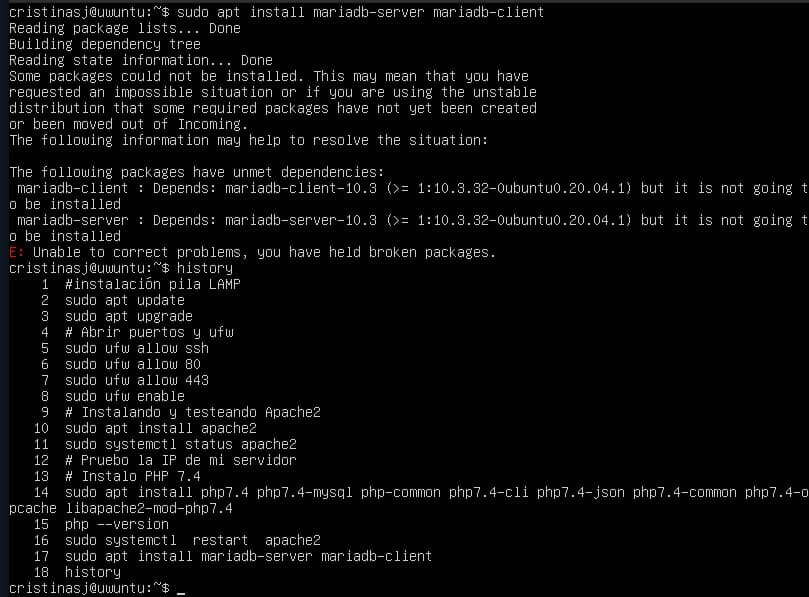
\includegraphics{mariaerror.jpg}
\end{figure} 
Para solucionarlo voy a instalar MySQL en su lugar
\newline 
Para eso voy a utilizar las instrucciones de esta página: \url{https://www.digitalocean.com/community/tutorials/how-to-install-linux-apache-mysql-php-lamp-stack-on-ubuntu-20-04}
Me vuelve dar un error, esta vez al usar el script mysql secure installation
\begin{figure}[H]
\centering
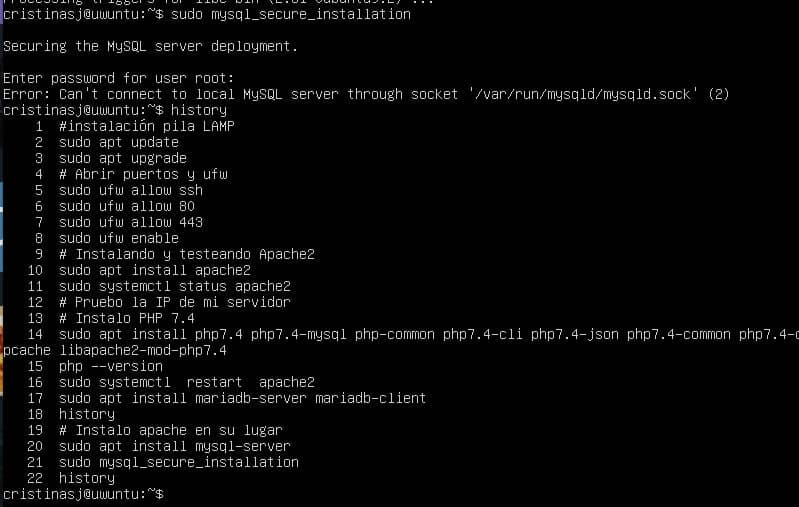
\includegraphics{sqlerror.jpg}
\end{figure}
La solución a este problema va a ser asumir que el servidor como viene por defecto es lo suficientemente seguro  
\newline
Ahora sí, voy a ponerme con la instalación de Zabbix. Mi primera fuente de información ha sido la página recomendada en las prácticas \url{https://www.zabbix.com/documentation/5.0/en/manual} 
\newline
En ella me llama la atención decargar zabbox desde la distribuición pre-compilada de la página web de Zabbix pero desde la máquina virtual no tengo esa opción así que deberé utilizar otra. 
\newline
Como segunda opción me baso en la documentación oficial. \url{https://www.zabbix.com/download?zabbix=5.0&os_distribution=ubuntu&os_version=20.04_focal&db=mysql&ws=apache} donde sí hay instrucciones para instalar en un servidor. 
\newline
Escribo el sigiente comando en ubuntu pero me da error: 
wget \url{https://repo.zabbix.com/zabbix/5.0/ubuntu/pool/main/z/zabbix-release/zabbix-release_5.0-1+focal_all.deb}
\newline
Me da un error:
\begin{figure}[H]
\centering
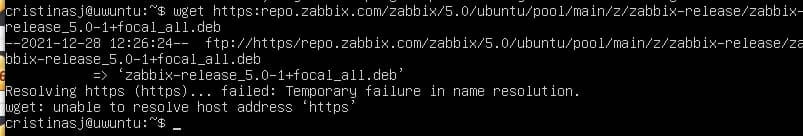
\includegraphics{Error1.jpg}
\end{figure} 
Tiene que haber sido un error de copiar porque lo vuelvo a intentar y ya funciona.
Sigo ejecutando los comandos: 
\begin{figure}[H]
\centering
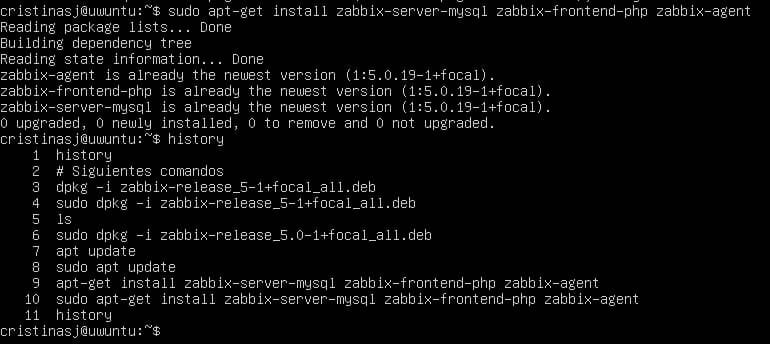
\includegraphics{instalacionhecha.jpg}
\end{figure} 


\subsection{Monitorización}
\subsubsection{A él mismo}
SSH y HTTP
\subsubsection{Máquina con CentOS}
\newpage
\end{document}
